\documentclass[11pt]{article}
\usepackage[utf8]{inputenc}
\usepackage[french]{babel}
\usepackage{graphicx}
\usepackage{caption}
\usepackage{fancyhdr} 
\usepackage{float}
\usepackage{lastpage}
\usepackage{amsmath}
\usepackage{amsfonts}
\usepackage{graphicx}
\usepackage{subcaption}
\usepackage{todonotes}
\usepackage{tikz}
\usepackage{listings}

\graphicspath{{./Images/}}

\renewcommand{\thesection}{\Roman{section}. }
\renewcommand{\thesubsection}{\Roman{section}.\arabic{subsection}}
\renewcommand{\thesubsubsection}{\Roman{section}.\arabic{subsection}.\alph{subsubsection} }

%%%%%%%%%%% Listings parameters %%%%%%%%%%

\lstdefinelanguage{JavaScript}{
  keywords={break, case, catch, continue, debugger, default, delete, do, else, false, finally, for, function, if, in, instanceof, new, null, return, switch, this, throw, true, try, typeof, var, void, while, with},
  morecomment=[l]{//},
  morecomment=[s]{/*}{*/},
  morestring=[b]',
  morestring=[b]",
  ndkeywords={class, export, boolean, throw, implements, import, this},
  sensitive=true
}

\lstset{
   language=JavaScript,
   backgroundcolor=\color{lightgray},
   extendedchars=true,
   basicstyle=\footnotesize\ttfamily,
   showstringspaces=false,
   showspaces=false,
   numbers=left,
   numberstyle=\footnotesize,
   numbersep=9pt,
   tabsize=2,
   breaklines=true,
   showtabs=false,
   captionpos=b
}

%%%%%%%%%%% Page style %%%%%%%%%%%%
\setlength{\hoffset}{-18pt}
\setlength{\oddsidemargin}{0pt}
\setlength{\evensidemargin}{0pt}
\setlength{\marginparwidth}{54pt}
\setlength{\textwidth}{494pt}
\setlength{\voffset}{-45pt}
\setlength{\marginparsep}{7pt}
\setlength{\topmargin}{0pt}
\setlength{\headheight}{13pt}
\setlength{\headsep}{15pt}
\setlength{\textheight}{680pt}

\pagestyle{fancy}

\renewcommand{\headrulewidth}{1pt}
\fancyhead[L]{\textsc{Génération Procédurale}}
\fancyhead[C]{}
\fancyhead[R]{\leftmark}

\renewcommand{\footrulewidth}{1pt}
\fancyfoot[L]{Rapport de projet}
\fancyfoot[C]{\textbf{\thepage/\pageref{LastPage}}}
\fancyfoot[R]{Equipe 12818}


\title{Rapport Projet}
\author{\textsc{Marais} Lucas, \textsc{Boudeau} Benjamin}
\date{2020-2021}


\begin{document}



\begin{titlepage}
\centering

\includegraphics[scale=0.3]{enseirb.png}
\\
\vspace*{1\baselineskip}
\LARGE{\textsc{Rapport de projet}}
\vspace*{0.8\baselineskip}
\rule{1\linewidth}{1pt}

\huge{\textbf{G\'EN\'ERATION PROC\'EDURALE}}
\vspace*{1\baselineskip}
\rule{1\linewidth}{1pt}
\vspace*{1\baselineskip}
\LARGE{\textsc{Filière Informatique - Semestre 6}}
\\

\large{\today}
\vspace*{3\baselineskip}
\\
\centering
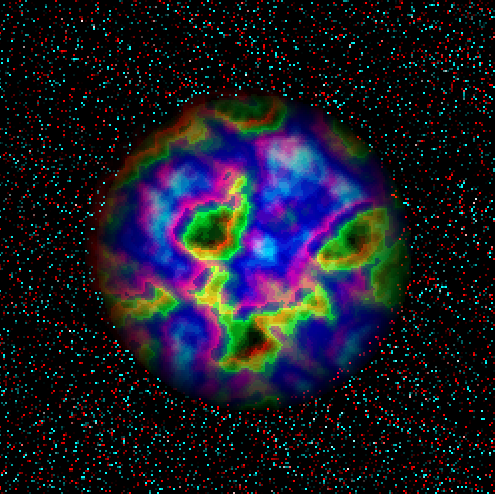
\includegraphics[scale=0.7]{planet.png}
\\
\vspace*{4\baselineskip}

\begin{minipage}[b]{0.40\linewidth}
        \flushleft 
        \large
        Auteurs : 
        \\
        \textsc{Choura} Alexandre
        \\
        \textsc{Guerin} Léo
        \\
        \textsc{Marais} Lucas
        \\
        \textsc{Sornay} Jean-François
    \end{minipage} \hfill
    \begin{minipage}[b]{0.40\linewidth}
        \flushright 
        \large 
        Encadrants : 
        \\
        \textsc{Renault} David
        \\
        \textsc{Rollet} Antoine
    \end{minipage} \hfill

\end{titlepage}

\newpage

%\section*{Introduction}


%\newpage

\tableofcontents




\newpage
\section{Introduction}
\label{section:introduction}

Le but de ce projet est, au travers de la réalisation d'une bibliothèque de fonctions de génération, transformation et composition de textures, de mettre en pratique les différentes notions de programmation fonctionnelle que nous avons pu apprendre lors de ce semestre. \\

Dans un premier temps, nous analyserons, dans ce rapport, les choix envisagées de représentations d'une image, de sa création ainsi que de sa modification. Dans un second temps, nous présentons les différents générateurs mis en place ainsi que les différents filtres conçus dans un troisième temps. Nous évoquerons dans un quatrième temps, notre méthodologie de tests. Enfin, dans un dernier temps, nous expliquerons brièvement comment nous nous sommes organisés tout au long de ce projet.

\vspace{15mm}
\section{Choix de représentation}
\label{section:representation}
L'une des premières étapes essentielles de ce projet fut le choix de la représentation d'une texture, de sa création à sa possible modification. Nous les présentons dans cette partie en commençant par la représentation que nous avons choisie, en passant par la représentation des générateurs de textures et par celle des filtres.

\subsection{Représentation d'une image}

Afin de représenter une image de manière fonctionnelle, la décision prise a été d'utiliser une fonction formalisée et d'ordre supérieur. Ainsi, nos images consistent à utiliser une fonction attribuant à chaque coordonnées $x, y \in \mathbb{R}_{+}$ une couleur de la forme d'un pixel RGBA, permettant alors de réaliser la texture désirée en calculant les pixels respectifs à chaque couple de coordonnées. Un avantage de cette représentation est que nous pouvons seulement évaluer une partie précise de l'image ou quelques pixels. De plus l'évaluation du pixel n'est effectuée qu'au dernier moment.



\subsection{Représentation d'un générateur}

Pour représenter un générateur de manière fonctionnelle, la décision prise a été d'utiliser des fonctions formalisées et d'ordre supérieur. Ainsi, nos générateurs consistent à prendre un objet représentant les options permettant de le configurer - sous la forme d'un dictionnaire similaire au format JSON - et retourne une fonction qui permet d'attribuer à chaque coordonnées une couleur de la forme d'un pixel RGBA. Ce pixel contient alors les informations de couleurs (rouge, vert, bleu) et de transparence (alpha) tel qu'expliqué dans la partie précédente.



\subsection{Représentation d'un filtre}

Notre vision d'un filtre ressemble fortement à celle d'un générateur. Ainsi, nos filtres consistent à prendre un objet représentant les options permettant de le configurer - dont au moins une d'elles est une image - et retourne une fonction qui permet d'attribuer à chaque coordonnées une couleur de la forme d'un pixel RGBA. \\

Cette fonctionnalité des filtres permet alors d'itérer plusieurs filtres les uns à la suite des autres. En effet, le fait de ne travailler qu'avec des fonctions nous permet alors, à partir d'une fonction génératrice d'image, d'appliquer un filtre, sur un filtre, sur un filtre, et ainsi de suite.

\newpage
\section{Générateurs}
\label{section:generators}

Dans le cadre de ce projet de programmation fonctionnelle, différents générateurs ont été implémentés. L'ensemble de ces générateurs permettent ainsi la génération de texture basées sur le bruit spatial, les pavages et certains plus particuliers. L'utilisation de ces derniers à travers la fonction de génération \texttt{generate} d'ordre supérieur, permet ainsi une inter-compatibilité entre filtres et générateurs. Cette dernière est présentée dans la sous-partie \ref{sec:generate}.

\subsection{Génération de bruit spatial}
\label{section:noiseGenerationIntro}

Dans le cadre de la génération de bruit spatial, quatres modules ont été réalisés:
\begin{itemize}
    \item [$\bullet$] \texttt{perlinNoiseGenerator}, permettant la génération de bruit de Perlin et ses variantes;
    \item [$\bullet$] \texttt{fractalNoiseGenerator}, permettant la génération de bruit fractal et ses variantes;
    \item [$\bullet$] \texttt{worleyNoiseGenerator}, permettant la génération de bruit de Worley et ses variantes;
    \item [$\bullet$] \texttt{domainWarpingFractal}, permettant la génération de déformation fractal de bruit.
\end{itemize}

L'ensemble de ces modules permettent ainsi la génération de textures à travers la fonction pure et d'ordre supérieur \texttt{noiseGenerator}, prenant en paramètre un dictionnaire sous format JSON permettant la configuration des bruits. Cette dernière retourne alors une fonction permettant de définir cette génération. La fonction retournée n'est cependant pas pure, cette dernière dépendant de l'ordre d'exécution des coordonnées. En effet, en raison de la génération aléatoire de nombre évoluant à partir d'une seed, l'ordre d'exécution influe alors directement sur les nombres générés. 

Pour palier à cela, la solution aurait pu être d'utiliser une fonction de génération de nombre aléatoire prenant en paramètres les coordonnées $x,y\in \mathbb{R}_{+}$, afin d'obtenir une génération dépendant de ces dernières, et ainsi indépendante des exécutions précédentes. Cependant, l'utilisation de seed n'aurait alors pas été possible, ce qui aurait limité la diversité de textures.

\subsubsection{Bruit de Perlin et variantes}
\label{section: perlinNoise}

\begin{figure}[H]
    \centering
    \begin{subfigure}{0.2\textwidth}
    \centering
            
\includegraphics[width=3cm]{PERLIN-VALUE-S1338.png}
        \caption{Bruit de valeur}
        \label{fig:perlinValueNoise}
    \end{subfigure}
    \begin{subfigure}{0.2\textwidth}
    \centering
        
\includegraphics[width=3cm]{PERLIN-GRADIENT-S1338.png}
        \caption{Bruit de gradient}
        \label{fig:perlinGradientNoise}
    \end{subfigure}
    \begin{subfigure}{0.2\textwidth}
    \centering
        
\includegraphics[width=3cm]{PERLIN-SIMPLEX-S1338.png}
        \caption{Bruit simplexe}
        \label{fig:perlinSimplexNoise}
    \end{subfigure}
    \caption{Exemples de bruit de Perlin générés à partir de la seed $1338$ par \texttt{perlinNoiseGenerator}}
    \label{fig:perlinNoise}
\end{figure}

Le bruit de Perlin s'articule en 3 sous-modules, représentés par
\begin{itemize}
    \item [$\bullet$] \texttt{valueNoise} pour le bruit de valeur, tel qu'illustré par la Figure \ref{fig:perlinValueNoise};
    \item [$\bullet$] \texttt{gradientNoise} pour le bruit de gradient, tel qu'illustré par la Figure \ref{fig:perlinGradientNoise};
    \item [$\bullet$] \texttt{simplexNoise} pour le bruit simplexe \cite{simplexNoise}, tel qu'illustré par la Figure \ref{fig:perlinSimplexNoise};
\end{itemize}

Cette organisation permet une implémentation indépendante de la variante choisie pour déterminer la valeur de bruit en utilisant \texttt{getNoiseHeight}, une fonction d'ordre supérieur. En effet, la variante choisie est chargée par la fonction pure et d'ordre supérieur \texttt{loadNoiseType}, renvoyant une fonction permettant de déterminer le bruit respectif à la variante pour un couple de coordonnées $x, y \in \mathbb{R}_{+}$ d'entrée. Chacune des variantes consiste à renvoyer une fonction \texttt{compute<Nom\_de\_la\_variante>} permettant de générer, par rapport aux paramètres d'entrées, pour tout $x, y \in \mathbb{R}_{+}$, une valeur de bruit correspondant aux propriétés de la variante souhaitée.


La génération de bruit de Perlin, orchestrée par la fonction d'ordre supérieur \texttt{perlinNoiseGenerator}, est pure, i.e., avec les mêmes paramètres d'entrée, l'on obtient toujours les mêmes résultats et elle n'a pas d'effets de bords avec son environnement extérieur. Par ailleurs, cette génération exploite l'utilisation interne d'un cache \texttt{gradients} permettant une génération plus rapide de la texture, afin d'éviter des calculs équivalents et inutiles de vecteurs précédemment calculés. Ainsi, s'il n'y avait pas eu d'utilisation de ce cache (ce qui n'aurait pas changer le comportement final de la génération), alors l'ensemble des fonctions composant la génération des variantes de bruit de Perlin serait lui aussi pure, car les fonctions n'auraient alors plus de contact avec leur environnement externe.

La génération d'images telles que celles de la Figure \ref{fig:perlinNoise} est permise par la fonction d'ordre supérieure \texttt{getPixelColor} retournée par la génération de bruit de Perlin, retournant un pixel RGBA pour un couple de coordonnées $x, y \in \mathbb{R}_{+}$ d'entrée en exploitant la fonction de retour de \texttt{getNoiseHeight}. Cette combinaison de fonctions, valeurs et opérateurs conjointement évalués permet de produire la texture finale.

Cette génération peut être configurée par un ensemble d'options donnée en entrée de \\ \texttt{perlinNoiseGenerator} sous la forme d'un dictionnaire. Les paramètres utilisés de ce dernier objet peuvent alors être
\begin{itemize}
    \item [$\bullet$] un nombre \texttt{seed}, afin d'initialiser la génération pseudo-aléatoire;
    \item [$\bullet$] \texttt{variant}, afin de choisir la variante à utiliser parmi \textit{value, gradient} et \textit{simplex};
    \item [$\bullet$] un nombre \texttt{scale}, afin de rétrécir/agrandir le zoom de la texture;
    \item [$\bullet$] un booléen \texttt{colored}, afin d'avoir une image colorée;
    \item [$\bullet$] un booléen \texttt{get\_noise}, afin d'avoir pour fonction de retour celle retournant une valeur de bruit à la place de celle retournant un pixel RGBA.
\end{itemize}
Ces paramètres sont tous optionnels, ces derniers étant initialement attribués une valeur par défaut.

\subsubsection{Bruit fractal et variantes}
\label{section: fractalNoise}

\begin{figure}[H]
    \centering
    \begin{subfigure}{0.2\textwidth}
    \centering
            
\includegraphics[width=3cm]{FBM-GRADIENT-O1-P05-L2-IA2-IF1-S2567.png}
        \caption{Octave $1$}
        \label{fig:fbmGradientO1}
    \end{subfigure}
    \begin{subfigure}{0.2\textwidth}
    \centering
        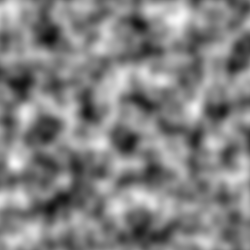
\includegraphics[width=3cm]{FBM-GRADIENT-O2-P05-L2-IA2-IF1-S2567.png}
        \caption{Octave $2$}
        \label{fig:fbmGradientO2}
    \end{subfigure}
    \begin{subfigure}{0.2\textwidth}
    \centering
        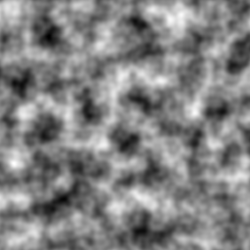
\includegraphics[width=3cm]{FBM-GRADIENT-O3-P05-L2-IA2-IF1-S2567.png}
        \caption{Octave $3$}
        \label{fig:fbmGradientO3}
    \end{subfigure}
    \begin{subfigure}{0.2\textwidth}
    \centering
        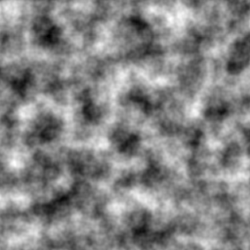
\includegraphics[width=3cm]{FBM-GRADIENT-O4-P05-L2-IA2-IF1-S2567.png}
        \caption{Octave $4$}
        \label{fig:fbmGradientO4}
    \end{subfigure}
    \caption{Exemples de Fractional Brownian Motion Noise de bruit de Perlin générés à partir de la variante du bruit de gradient, de persistence $0.5$, lacunarité $2$, amplitude initiale $2$, fréquence initiale $1$ et seed $2567$, par \texttt{fractalNoiseGenerator}}
    \label{fig:fbmGradient}
\end{figure}

\begin{figure}[H]
    \centering
    \begin{subfigure}{0.2\textwidth}
    \centering
            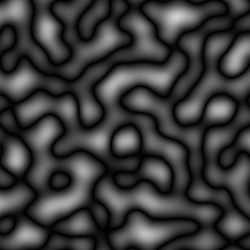
\includegraphics[width=3cm]{TURBULENCE-GRADIENT-O1-P05-L2-IA2-IF1-S2567.png}
        \caption{Octave $1$}
        \label{fig:turbulenceGradientO1}
    \end{subfigure}
    \begin{subfigure}{0.2\textwidth}
    \centering
        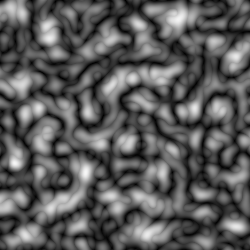
\includegraphics[width=3cm]{TURBULENCE-GRADIENT-O2-P05-L2-IA2-IF1-S2567.png}
        \caption{Octave $2$}
        \label{fig:turbulenceGradientO2}
    \end{subfigure}
    \begin{subfigure}{0.2\textwidth}
    \centering
        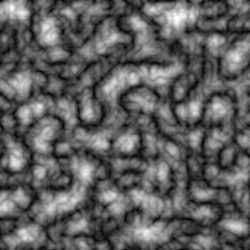
\includegraphics[width=3cm]{TURBULENCE-GRADIENT-O3-P05-L2-IA2-IF1-S2567.png}
        \caption{Octave $3$}
        \label{fig:turbulenceGradientO3}
    \end{subfigure}
    \begin{subfigure}{0.2\textwidth}
    \centering
        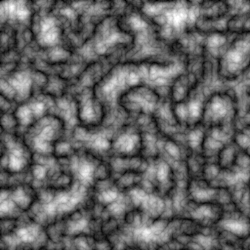
\includegraphics[width=3cm]{TURBULENCE-GRADIENT-O4-P05-L2-IA2-IF1-S2567.png}
        \caption{Octave $4$}
        \label{fig:turbulenceGradientO4}
    \end{subfigure}
    \caption{Exemples de Turbulence Noise de bruit de Perlin générés à partir de la variante du bruit de gradient, de persistence $0.5$, lacunarité $2$, amplitude initiale $2$, fréquence initiale $1$ et seed $2567$, par \texttt{fractalNoiseGenerator}}
    \label{fig:turbulenceGradient}
\end{figure}

\begin{figure}[H]
    \centering
    \begin{subfigure}{0.2\textwidth}
    \centering
            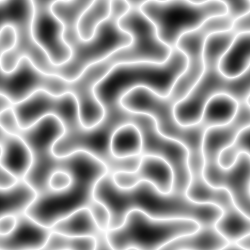
\includegraphics[width=3cm]{RIDGED-GRADIENT-O1-P05-L2-IA2-IF1-S2567.png}
        \caption{Octave $1$}
        \label{fig:ridgedGradientO1}
    \end{subfigure}
    \begin{subfigure}{0.2\textwidth}
    \centering
        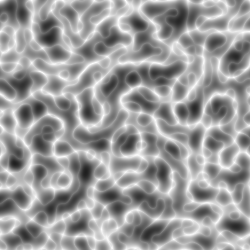
\includegraphics[width=3cm]{RIDGED-GRADIENT-O2-P05-L2-IA2-IF1-S2567.png}
        \caption{Octave $2$}
        \label{fig:ridgedGradientO2}
    \end{subfigure}
    \begin{subfigure}{0.2\textwidth}
    \centering
        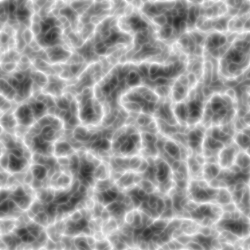
\includegraphics[width=3cm]{RIDGED-GRADIENT-O3-P05-L2-IA2-IF1-S2567.png}
        \caption{Octave $3$}
        \label{fig:ridgedGradientO3}
    \end{subfigure}
    \begin{subfigure}{0.2\textwidth}
    \centering
        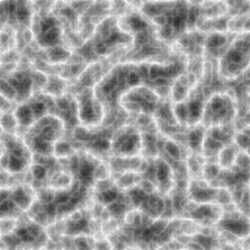
\includegraphics[width=3cm]{RIDGED-GRADIENT-O4-P05-L2-IA2-IF1-S2567.png}
        \caption{Octave $4$}
        \label{fig:ridgedGradientO4}
    \end{subfigure}
    \caption{Exemples de Ridged Noise de bruit de Perlin générés à partir dela variante du bruit de gradient, de persistence $0.5$, lacunarité $2$, amplitude initiale $2$, fréquence initiale $1$ et seed $2567$, par \texttt{fractalNoiseGenerator}}
    \label{fig:ridgedGradient}
\end{figure}

Le principe d'un bruit fractal est d'accumuler plusieurs valeurs de bruit d'un même type, permettant l'obtention de nouveaux effets ou détails par rapport au bruit initial, telle que le montre les Figures \ref{fig:fbmGradient}, \ref{fig:turbulenceGradient} et \ref{fig:ridgedGradient}. On parle alors d'octave pour chaque nouvelle couche ou superposition de ces valeurs de bruit. \cite{fractalNoise}

La génération de bruit fractal se base sur les fonctions de retour des modules de génération de bruit de Perlin \ref{section: perlinNoise} et de Worley \ref{section: worleyNoise}. Ainsi, en utilisant l'option \texttt{get\_noise} de ces deux derniers, la génération de bruit fractal exploite leur fonction \texttt{getNoiseHeight}, renvoyant une valeur de bruit. Cet aspect a été utilisé afin d'obtenir un ensemble de générateur pour chaque octaves à travers \texttt{getOctaveGenerator}, une fonction pure et d'ordre supérieur, renvoyant un tableau de fonction (correspondant à \texttt{getNoiseHeight}) permettant d'obtenir le bruit relatif à un couple de coordonnées $x, y \in \mathbb{R}_{+}$ d'entrée pour chaque octaves.

Par ailleurs, de notre propre initiative, nous avons implémenté différentes variantes de bruit fractal:
\begin{itemize}
    \item [$\bullet$] Une première correspondant à une notion de \textit{Fractal Brownian Motion}, permettant un rendu tel qu'illustré par la Figure \ref{fig:fbmGradient}. C'est la génération classique de bruit fractal multipliant la valeur de bruit de chacun des octaves par l'amplitude de ce dernier;
    \item [$\bullet$] Une deuxième correspondant à une notion de \textit{Turbulence}, permettant un rendu tel qu'illustré par la Figure \ref{fig:turbulenceGradient}. Cette génération diffère par l'utilisation de la valeur absolue de la valeur de bruit de chacun des octaves;
    \item [$\bullet$] Une deuxième correspondant à une notion de \textit{Ridged}, permettant un rendu tel qu'illustré par la Figure \ref{fig:ridgedGradient}. Cette génération diffère par l'utilisation de la valeur absolue de la valeur de bruit soustrait à 1 élevé au carré pour chacun des octaves.
\end{itemize}

Il est aisé de remarquer que ces variantes sont très similaires algorithmiquement, et que la seule différence réside dans la manière dont le bruit de chaque octave est traitée et accumulée. Ainsi, afin de rendre le code et l'implémentation de bruits fractals plus fonctionnels, avoir un algorithme d'accumulation plus simple et indépendant de la variante choisie et éviter une duplication de code inutile (et n'exploitant pas les capacités fonctionnelles de JavaScript), la fonction d'ordre supérieur \texttt{getNoiseHeight} permettant d'obtenir la valeur finale de bruit prend en entrée la fonction définissant la transformation à appliquer, ainsi que ses états initiaux de bruits, d'amplitude et de fréquence, et ses multiplicateurs. Cela est notamment rendu possible par la fonction d'ordre supérieur \texttt{loadArgFractalGen}, renvoyant la hauteur de bruit initial et la transformation à appliquer à chaque octave, en fonction de la variante d'entrée.

Il est important de noter que les fonctions \texttt{loadArgFractalGen}, \texttt{getNoiseHeight} et \texttt{getPixelColor} composant la génération de bruit fractal ne sont pas pures. En effet, afin d'avoir un rendu visuel final optimal, des effets de bords sont réalisés afin de rendre compte des bornes des valeurs de bruits obtenues. Ce choix permet d'avoir une texture finale plus contrastée, en actualisant ces bornes à la fin de chaque appel à \texttt{getNoiseHeight} en comparant la valeur de bruit obtenu pour un couple de coordonnées $x, y \in \mathbb{R}_{+}$ d'entrée aux extremums. Cela aura pour effet d'homogénéiser le bruit final, en le mettant à l'échelle en fonction de ses bornes. Cependant, si ce choix n'avait pas été effectué, alors l'ensemble des fonctions composant le module \texttt{fractalNoiseGenerator} serait purs, car leurs résultats seraient alors indépendants des conditions extérieures et résultats antérieurs, et ne dépendraient plus qu'uniquement de leurs paramètres d'entrée.

Ainsi, en exploitant les notions de programmation fonctionnelle et les capacités de JavaScript, le générateur de bruit fractal est alors simple, court à écrire et générique. Cette génération peut être configurée par un ensemble d'options donnée en entrée de \texttt{perlinNoiseGenerator} sous la forme d'un dictionnaire. Les paramètres utilisés de ce dernier objet peuvent alors être
\begin{itemize}
    \item [$\bullet$] \texttt{fractal}, afin de déterminer le type de bruit fractal à générer;
    \item [$\bullet$] \texttt{noiseGen}, afin de déterminer le type de bruit à utiliser parmis \textit{perlin} et \textit{worley};
    \item [$\bullet$] un nombre \texttt{seed}, afin d'initialiser la génération pseudo-aléatoire;
    \item [$\bullet$] un dictionnaire d'options \texttt{argsList} afin de paramétrer la génération de bruit;
    \item [$\bullet$] un nombre \texttt{octaves} afin de déterminer le nombre d'octaves à superposer;
    \item [$\bullet$] un nombre \texttt{persistence} afin de fixer le multiplicateur de l'amplitude pour chaque octaves;
    \item [$\bullet$] un nombre \texttt{lacunarity} afin de fixer le multiplicateur de la fréquence pour chaque octaves;
    \item [$\bullet$] un nombre \texttt{initial\_amplitude} afin de fixer l'amplitude initial au premier octave;
    \item [$\bullet$] un nombre \texttt{initial\_frequency} afin de fixer la fréquence initial au premier octave;
    \item [$\bullet$] un booléen \texttt{colored}, afin d'avoir une image colorée;
    \item [$\bullet$] un booléen \texttt{get\_noise}, afin d'avoir pour fonction de retour celle retournant une valeur de bruit à la place de celle retournant un pixel RGBA.
\end{itemize}
Ces paramètres sont tous optionnels, ces derniers étant initialement attribués à une valeur par défaut.

\begin{figure}[H]
    \centering
    \begin{subfigure}{0.2\textwidth}
    \centering
            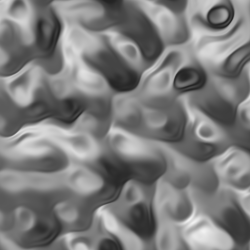
\includegraphics[width=3cm]{WARP-FBM-GRADIENT-O1-P05-L2-IA2-IF1-S2567-Q40-R20.png}
        \caption{Octave $1$}
        \label{fig:warpFbmGradientO1}
    \end{subfigure}
    \begin{subfigure}{0.2\textwidth}
    \centering
        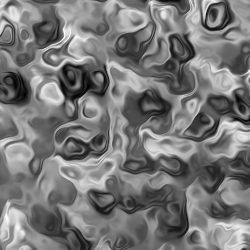
\includegraphics[width=3cm]{WARP-FBM-GRADIENT-O2-P05-L2-IA2-IF1-S2567-Q40-R20.png}
        \caption{Octave $2$}
        \label{fig:warpFbmGradientO2}
    \end{subfigure}
    \begin{subfigure}{0.2\textwidth}
    \centering
        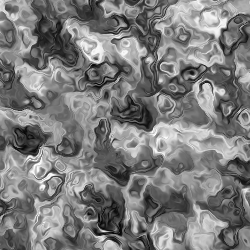
\includegraphics[width=3cm]{WARP-FBM-GRADIENT-O3-P05-L2-IA2-IF1-S2567-Q40-R20.png}
        \caption{Octave $3$}
        \label{fig:warpFbmGradientO3}
    \end{subfigure}
    \begin{subfigure}{0.2\textwidth}
    \centering
        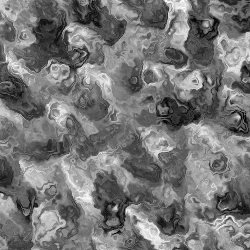
\includegraphics[width=3cm]{WARP-FBM-GRADIENT-O4-P05-L2-IA2-IF1-S2567-Q40-R20.png}
        \caption{Octave $4$}
        \label{fig:warpFbmGradientO4}
    \end{subfigure}
    \caption{Exemples de Domain Warping de bruit fractal de bruit de Perlin générés à partir de la variante du bruit de gradient, de persistance $0.5$, lacunarité $2$, amplitude initiale $2$, fréquence initiale $1$, seed $2567$, multiplicateur q de $40$ et r de $20$, par \texttt{domainWarpingFractalGenerator}}
    \label{fig:warpFbmGradient}
\end{figure}

Suite à la réalisation de ce module permettant la génération de bruit fractal, la prochaine étape fut naturellement l'implémentation de \textit{Fractal Domain Warping} \cite{fractalDomainWarping}. Cette génération, telle qu'illustrée par la Figure \ref{fig:warpFbmGradient}, repose sur la composition de bruits fractals afin de créer un effet de déformation spatiale. Ainsi, \texttt{domainWarpingFractalGenerator} permet la génération d'une telle texture en mettant à profit la fonction de retour de \texttt{fractalNoiseGenerator} en utilisant l'option \texttt{get\_noise}, permettant alors d'obtenir une valeur de bruit dans l'intervalle $]-1;1[$. Finalement, afin de générer un bruit issu de Fractal Domain Warping, il a alors simplement suffi de composer les fractales \cite{fractalDomainWarping}, permettant ainsi d'obtenir une valeur de bruit grâce à une fonction d'ordre supérieur prenant en paramètre la fonction \texttt{fractal} à utiliser, ce qui permet d'aboutir à la texture souhaitée.

Cette génération peut être configurée par un ensemble d'options donnée en entrée de\\ \texttt{domainWarpingFractalGenerator} sous la forme d'un dictionnaire. Les paramètres utilisées de ce dernier objet peuvent alors être ceux décrivant un bruit fractal, ainsi que
\begin{itemize}
    \item [$\bullet$] un nombre \texttt{qMultiplier} permettant de définir le premier niveau de distorsion;
    \item [$\bullet$] un nombre \texttt{rMultiplier} permettant de définir le second niveau de distorsion;
    \item [$\bullet$] un booléen \texttt{colored}, afin d'avoir une image colorée;
    \item [$\bullet$] un booléen \texttt{get\_noise}, afin d'avoir pour fonction de retour celle retournant une valeur de bruit à la place de celle retournant un pixel RGBA.
\end{itemize}
Ces paramètres sont tous optionnels, ces derniers étant initialement attribués à une valeur par défaut.

\subsubsection{Bruit de Worley et variantes}
\label{section: worleyNoise}

\begin{figure}[H]
    \centering
    \begin{subfigure}{0.2\textwidth}
    \centering
            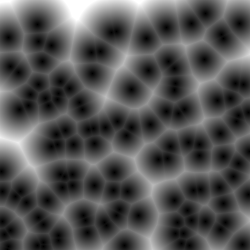
\includegraphics[width=3cm]{WORLEY-F1-EUCLIDEAN-3DOFF-S43-NPWIDTH2.png}
        \caption{Type F1 avec distance euclidienne en 2D avec la seed 43 et $\frac{\texttt{width}}{2}$ points}
        \label{fig:worleyF1euclidean}
    \end{subfigure}
    \begin{subfigure}{0.2\textwidth}
    \centering
        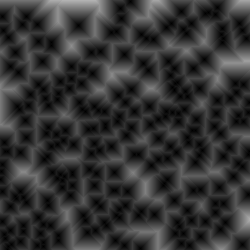
\includegraphics[width=3cm]{WORLEY-F1-CHEBYSHEV-3DOFF-S43-NPWIDTH.png}
        \caption{Type F1 avec distance de chebyshev en 2D avec la seed 43 et \texttt{width} points}
        \label{fig:worleyF1chebyshev}
    \end{subfigure}
    \begin{subfigure}{0.2\textwidth}
    \centering
        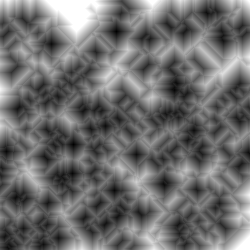
\includegraphics[width=3cm]{WORLEY-F2-MANHATTAN-3DOFF-S43-NPWIDTH.png}
        \caption{Type F2 avec distance de manhattan en 2D avec la seed 43 et \texttt{width} points}
        \label{fig:worleyF2manhattan}
    \end{subfigure}
    \begin{subfigure}{0.2\textwidth}
    \centering
        
\includegraphics[width=3cm]{WORLEY-F2F1-EUCLIDEAN-3DON-S43-CLRD.png}
        \caption{Type F2-F1 avec distance euclidean en 3D colorisé avec la seed 43}
        \label{fig:worleyF2F1euclidean}
    \end{subfigure}
    \caption{Exemples de bruit de Worley générés par \texttt{worleyNoiseGenerator}, de taille $250$x$250$}
    \label{fig:worley}
\end{figure}

Le principe de la génération de bruit de Worley est simple. Il consiste à calculer, pour un couple de coordonnées $x, y \in \mathbb{R}_{+}$ d'entrée, la distance aux points de référence statiques. La génération de bruit de Worley, telle qu'illustrée par la Figure \ref{fig:worley}, exploite au maximum les principes de la programmation fonctionnelle afin d'obtenir un code générique dans son algorithmique, et simple dans sa compréhension. Ainsi, une majeure partie de l'implémentation du bruit de Worley réside dans l'initialisation des différentes fonctions qui vont permettre l'évaluation des distances.

\begin{figure}[H]
    \centering
    \begin{tikzpicture}[sibling distance=15em, scale=0.80,
        every node/.style = {shape=rectangle, rounded corners,
        draw, align=center, scale=0.80,
        top color=white, bottom color=blue!20}]]
    \node {\texttt{getPixelColor}}
    child { node { \texttt{getDist} }
        child { node { \texttt{loadArgType} } 
            child { node { \texttt{getNthNearestDistance} } 
                child { node { \texttt{distanceDimension} } 
                    child { node { \texttt{distanceFormulas} }
                        child { node { \texttt{loadArgDistance} } 
                            child { node { \texttt{getDistanceChebyshev} \\ \texttt{getDistanceManhattan} \\ \texttt{getDistanceEuclidean}} 
                                child { node { \texttt{two\_dim: getDistance2D} } } 
                                child { node { \texttt{three\_dim: getDistance3D}} }
                            }
                        }
                    }
                }
                child { node { \texttt{featurePoints} } 
                    child { node { \texttt{generateFeaturePoints} } 
                        child { node { \texttt{makeRandom} } }
                    }
                }
            }    
        }
    };
    \end{tikzpicture}
    \caption{Graphe de dépendance des fonctions ou constantes (passées en paramètres) du bruit de Worley}\label{fig:graphWorley}
\end{figure}

Lors des explications suivantes, la Figure \ref{fig:graphWorley} permettra de servir d'appui à la compréhension. Initialement, il faut répartir les points de référence statiques dans l'espace. Cette tâche triviale est réalisé par \texttt{generateFeaturePoints}, une fonction pure et d'ordre supérieur retournant un tableau de positions. Ces positions sont alors stockées dans la constante \texttt{featurePoints}.

D'une part, il faut pouvoir définir la formule de distance à utiliser, i.e., \textit{euclidienne} (Figure \ref{fig:worleyF1euclidean}), de \textit{chebyshev} (Figure \ref{fig:worleyF1chebyshev}) ou de \textit{manhattan} (Figure \ref{fig:worleyF2manhattan}). C'est ainsi que trois modules de distances ont été implémentés (\texttt{getDistanceChebyshev}, \texttt{getDistanceManhattan} et \texttt{getDistanceEuclidean}), retournant les formules permettant de calculer la distance entre deux points en 2D (resp. 3D) à travers \texttt{getDistance2D} (resp. \texttt{getDistance3D}) obtenable par l'option \texttt{two\_dim} (resp. \texttt{three\_dim}) de l'objet retourné. Ainsi, les formules susceptibles d'être utilisé par rapport aux type de calcul de distance souhaité sont chargées par \texttt{loadArgDistance}, qui retourne alors le dictionnaire contenant les formules 2D et 3D. Par la suite, et en fonction des paramètres d'entrées du générateur, la distinction est faite en choisissant la dimension du calcul de distance souhaitée. Ces étapes effectuées, la formule à utiliser est alors représentée par la constante \texttt{distanceDimension}.

D'autre part, il faut pouvoir définir l'expression du calcul à effectuer. Pour aider à la compréhension, \textit{f\textbf{X}} représentera la \textbf{X}ème distance la plus proche aux points de référence statiques. Ainsi, les différentes expressions possibles sont \textit{f2-f1} (Figure \ref{fig:worleyF2F1euclidean}), \textit{f2} (Figure \ref{fig:worleyF2manhattan}) ou \textit{f1} (Figure \ref{fig:worleyF1euclidean}). Ainsi, le type d'expression à utiliser est obtenu grâce à la fonction \texttt{loadArgType}, retournant une fonction currifiée permettant de définir, en fonction de la formule de distance, du nombre de points et de leurs positions, une expression permettant de calculer pour tout couple de coordonées $x, y \in \mathbb{R}_{+}$ d'entrée l'expression souhaitée, en utilisant \texttt{getNthNearestDistance}. Cette expression de fonction(s) est alors stockée dans une constante \texttt{getDist}.

Enfin, une fois toutes ces données initialisées, il suffit de faire appel à \texttt{getDist} afin de calculer l'évaluation des distances pour un point de coordonnées $(x, y)$. Après remise à l'échelle afin d'obtenir l'équivalent d'une valeur de bruit, on peut générer une texture à travers \texttt{getPixelColor}, une fonction d'ordre supérieur.

\begin{figure}[H]
    \centering
    \begin{subfigure}{0.2\textwidth}
    \centering
            
\includegraphics[width=3cm]{RIDGED-F2F1-DEUCLIDEAN-O1-3DON-P05-L2-IA2-IF05-S44-CLRD.png}
        \caption{Octave $1$}
        \label{fig:ridgedWorleyO1}
    \end{subfigure}
    \begin{subfigure}{0.2\textwidth}
    \centering
        
\includegraphics[width=3cm]{RIDGED-F2F1-DEUCLIDEAN-O2-3DON-P05-L2-IA2-IF05-S44-CLRD.png}
        \caption{Octave $2$}
        \label{fig:ridgedWorleyO2}
    \end{subfigure}
    \begin{subfigure}{0.2\textwidth}
    \centering
        
\includegraphics[width=3cm]{RIDGED-F2F1-DEUCLIDEAN-O3-3DON-P05-L2-IA2-IF05-S44-CLRD.png}
        \caption{Octave $3$}
        \label{fig:ridgedWorleyO3}
    \end{subfigure}
    \caption{Exemples de bruit fractal ridged de bruit de Worley générés à partir de la seed $44$, de persistence $0.5$, lacunarité $2$, amplitude initiale $2$, fréquence initiale $0.5$, en 3D colorisé, par \texttt{fractalNoiseGenerator}}
    \label{fig:ridgedWorley}
\end{figure}

Il est à noter que de manière similaire au bruit de Perlin, toutes les fonctions composant la génération du bruit de Worley auraient pu être pures s'il n'y avait pas eu l'utilisation d'un cache des distances calculées, ce qui permet de réduire le temps de génération. De la même manière, on peut alors obtenir des bruits fractals à partir de bruit de Worley, tel que le montre la figure \ref{fig:ridgedWorley} en appelant le générateur avec l'option \texttt{get\_noise}, qui renverra une fonction permettant de remettre à l'échelle une distance dans l'intervalle caractéristique d'un bruit $]-1;1[$. Cette génération fractale est cependant beaucoup plus lente, et $3$ octaves semble être le nombre de superposition raisonnable maximum pour cette génération (avec un processeur cadencé à $4.2$ GHz), voire $2$; un nombre supérieur n'apportant de toute manière que peu de détails supplémentaires, peu perceptibles. Par ailleurs, la génération de bruit de Worley sur des images de moyennes ou grandes dimensions est assez lente, voire trop lente, mais aurait pu être réduite drastiquement en effectuant un pavage du plan et en ne comparant les distances qu'aux voisins directs, au lieu de calculer les distances à tous les points représentatifs statiques. \cite{worleyNoise}

Cette génération peut être configurée par un ensemble d'options donnée en entrée de\\ \texttt{worleyNoiseGenerator} sous la forme d'un dictionnaire. Les paramètres utilisés de ce dernier objet peuvent alors être
\begin{itemize}
    \item [$\bullet$] un nombre \texttt{seed}, afin d'initialiser la génération pseudo-aléatoire;
    \item [$\bullet$] \texttt{type}, afin de choisir l'expression du calcul de distance à utiliser parmis \textit{f1, f2} et \textit{f2 - f1};
    \item [$\bullet$] \texttt{distance}, afin de choisir la formule de distance à utiliser parmis \textit{euclidean, manhattan} et \textit{chebyshev};
    \item [$\bullet$] un booléen \texttt{three\_dimensions}, afin d'avoir des calculs de distances en 3D;
    \item [$\bullet$] un booléen \texttt{colored}, afin d'avoir une image colorée;
    \item [$\bullet$] un nombre \texttt{number\_of\_points} permettant de fixer le nombre de points de références caractéristiques;
    \item [$\bullet$] un booléen \texttt{get\_noise}, afin d'avoir pour fonction de retour celle retournant une valeur de bruit à la place de celle retournant un pixel RGBA.
\end{itemize}
Ces paramètres sont tous optionnels, ces derniers étant initialement attribués une valeur par défaut.

\subsection{Génération de pavages}

La génération de pavages réguliers ou semi-réguliers repose en grande partie sur des propriétés géométriques. Afin de garantir un aspect fonctionnel, nous avons fait le choix d'avoir un ensemble de fonctions dans le fichier \texttt{GeometricPredicate.js} qui permet de vérifier des propriétés mathématiques et géométriques simples sur les variables passées en argument. Par exemple, nous avons des fonctions qui nous indiquent si un nombre est pair ou non, qui regarde si deux nombres ont la même parité ou si un point appartient à une certaine droite. Une fois ces fonctions misent en place nous avons développé les générateurs de pavages.

Les générateurs de pavages implémentés sont des constructeurs de fonctions pures. Ces constructeurs créent une fonction avec le paramétrage donné en argument et renvoient celle-ci. Cette fonction associe à chaque pixel une couleur en fonction de ses coordonnées. Il ne reste plus qu'à appliquer cette fonction sur chaque pixel pour générer le pavage. De plus, pour déterminer la couleur du pixel donné en entrée la fonction ne se base que sur ses coordonnées, donc la couleur résultante est indépendante de l'ordre d'application sur les différents pixels. De cette manière nous avons développé plusieurs générateurs de pavages réguliers et semi-réguliers. La figure \ref{fig:tiling} présente différentes images produites avec nos générateurs de pavages. 

\begin{figure}[H]
    \centering
    \begin{subfigure}{0.2\textwidth}
    \centering
            
\includegraphics[width=3cm]{Images/echiquier.png}
        \caption{Échiquier en version noir et blanc}
        \label{fig:echiquier}
    \end{subfigure}
    \begin{subfigure}{0.2\textwidth}
    \centering
        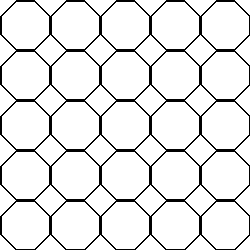
\includegraphics[width=3cm]{Images/octagonal.png}
        \caption{Pavage semi-régulier}
        \label{fig:octagonal}
    \end{subfigure}
    \begin{subfigure}{0.2\textwidth}
    \centering
        
\includegraphics[width=3cm]{Images/voronoi.png}
        \caption{Motif de \textit{Voronoi}}
        \label{fig:voronoi}
    \end{subfigure}
    \begin{subfigure}{0.2\textwidth}
        \centering
        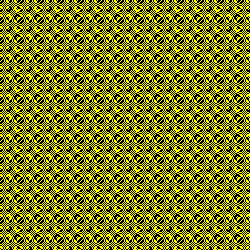
\includegraphics[width=3cm]{Images/bee.png}
        \caption{Motif en forme d'abeilles}
        \label{fig:bee}
    \end{subfigure}
    \caption{Exemples d'images générées avec nos générateurs de pavages}
    \label{fig:tiling}
\end{figure}

\subsection{Générateurs particuliers}

Dans cette sous-section, nous allons présenter un autre type de générateur que nous avons souhaité ajouter afin de pouvoir mettre en couleur un bruit quelconque à l'aide d'un gradient de couleurs.

\subsubsection{Gradients de couleurs}

Le but de nos générateurs de gradients de couleurs est de produire une carte de couleurs des variations d'un bruit quelconque. Pour cela nous avons d'abord écrit une fonction \texttt{multiGradient} qui prend en paramètre deux bornes d'un intervalle $I$ sur lequel nous souhaitons construire un gradient. Ensuite, la fonction \texttt{multiGradient} renvoie une fonction. Cette dernière prend en argument un ensemble de valeurs comprises entre $0$ et $255$ formant les variations du gradient de couleurs ainsi que la valeur du bruit en un point. Cette fonction retourne alors la valeur du gradient en ce point. 

Pour généraliser cela à une couleur RGBA, nous avons codé une fonction \texttt{colorMap} qui est aussi un constructeur de fonctions. Ce constructeur prend les bornes de l'intervalle $I$, les variations pour chaque composante de la couleur et une fonction bruit. La fonction \texttt{colorMap} retourne une fonction prenant des coordonnées en argument et renvoyant la couleur correspondante. Par exemple, pour produire un gradient en nuance de gris sur un intervalle de valeur comprises entre $0$ et $250$, il faut utiliser la fonction \texttt{colorMap} avec en paramètre les valeurs $0$,$250$ et $[[0,255]]$ pour les variations pour chaque couleur RGBA. Il faut aussi passer en paramètre une fonction de produisant un bruit comme la fonction $(x,y)=>x$. La figure \ref{fig:greys} correspond à l'image générée avec ces paramètres pour une image de taille $250X250$.

Un défaut de notre implémentation est le fait que cela peut être fastidieux de créer un gradient avec un grand nombre de variations de couleurs. Nous avons alors codé des constructeurs de gradients pré-paramétrés pour des variations de couleurs. Ces constructeurs prennent en argument les bornes de l'intervalle sur lequel appliquer le gradient et la fonction bruit. Le constructeur renvoie une fonction prenant des coordonnées en argument et retournant la couleur correspondante. Parmi ces exemples de gradients nous avons une carte de variations en nuances de gris, en plusieurs couleurs ainsi qu'en mode continue ou discontinue. La figure \ref{fig:colormap} présente différents exemples de gradients que nous avons implémentés.

\begin{figure}[H]
    \centering
    \begin{subfigure}{0.2\textwidth}
    \centering
            
\includegraphics[width=3cm]{Images/greys.png}
        \caption{Gradient en nuances de gris}
        \label{fig:greys}
    \end{subfigure}
    \begin{subfigure}{0.2\textwidth}
    \centering
        
\includegraphics[width=3cm]{Images/mushroom.png}
        \caption{Gradient du rouge vers le cyan}
        \label{fig:mushroom}
    \end{subfigure}
    \begin{subfigure}{0.2\textwidth}
    \centering
        
\includegraphics[width=3cm]{Images/island_discont.png}
        \caption{Exemple d'un gradient continu}
        \label{fig:gradient_continu}
    \end{subfigure}
    \begin{subfigure}{0.2\textwidth}
    \centering
        
\includegraphics[width=3cm]{Images/island_continu.png}
        \caption{Exemple d'un gradient discontinu}
        \label{fig:gradient_discontinu}
    \end{subfigure}
    \caption{Exemples de gradients de couleurs}
    \label{fig:colormap}
\end{figure}

\subsubsection{Fractales}

Afin de générer des figures de type fractal, nous avons mis en place un constructeur de fonctions générant des figures fractales. Ce constructeur prend en paramètre une fonction, une valeur frontière pour la figure, et le nombre d'appels récursifs terminaux à effectuer sur la fonction. 
La fonction génératrice ainsi retournée, produit un bruit fractal en fonction des coordonnées du pixel sur lequel elle est appelée. Ces fonctions ont besoin d'être passées en paramètre de nos gradients de couleurs pour produire une image. Pour avoir quelques exemples d'utilisation, nous avons ajouté des fonctions générant des figures fractales spécifiques. Par exemple, nous avons des fonctions produisant les figures de l'ensemble de \textit{Julia}. La figure \ref{fig:colormappred} présente différents exemples de fonctions générant une fractale associée à différents gradients de couleurs que nous avons implémentés.

\begin{figure}[H]
    \centering
    \begin{subfigure}{0.2\textwidth}
    \centering
        
\includegraphics[width=3cm]{Images/juliaDragon.png}
        \caption{Exemple de fractale de \textit{Julia}}
        \label{fig:juliaDragon}
    \end{subfigure}
    \begin{subfigure}{0.2\textwidth}
    \centering
        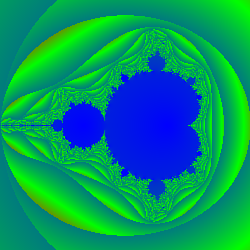
\includegraphics[width=3cm]{Images/mandelBrot.png}
        \caption{Fractale de \textit{Mandelbrot}}
        \label{fig:mandelbrot}
    \end{subfigure}
    \begin{subfigure}{0.2\textwidth}
    \centering
        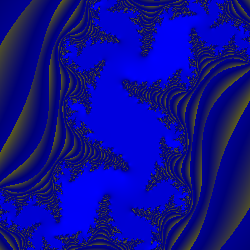
\includegraphics[width=3cm]{Images/juliaBubble.png}
        \caption{Autre exemple de fractale de \textit{Julia}}
        \label{fig:juliaBubble}
    \end{subfigure}
    \caption{Exemples de générateurs de figures fractales associé à différents gradients de couleurs}
    \label{fig:colormappred}
\end{figure}

\subsection{Composition de générateur : \textit{generate}}
\label{sec:generate}
Afin de faciliter la composition entre différents générateurs et filtres, nous avons mis au point une fonction \textit{generate} qui prend en paramètre un objet que nous avons appelé \textit{descriptor} possédant différents champs optionnels ou obligatoires. L'écriture de cet objet s'inspire du format JSON et possède les champs suivants :
\begin{itemize}
    \item \texttt{src} : Objet contenant les champs :
    \begin{itemize}
        \item [$\bullet$] \texttt{img} : Fonction génératrice de texture
        \item [$\bullet$] \texttt{options} : Options du générateur présent dans le champs \textit{img}
        \item [$\bullet$] \texttt{filters} : Objet étant utilisé comme un tableau de filtres à appliquer à la fonction génératrice du champ \textit{img}. Il possède un nombre quelconque de champs représentés par un nombre et étant un objet lui-même contenant :
        \begin{itemize}
            \item [$\circ$] \texttt{filter} : Fonction étant un filtre
            \item [$\circ$] \texttt{filter\_options} : Options du filtre
        \end{itemize}
    \end{itemize}
    \item \texttt{linker} : Objet permettant d'utiliser des compositions de générateurs :
    \begin{itemize}
        \item [$\bullet$] \texttt{composition} : Fonction de composition
        \item [$\bullet$] \texttt{options} : Options de la fonction de composition
    \end{itemize}
    \item \texttt{dst} : Objet de type \textit{descriptor}
    \item \texttt{filters} : Objet de même type que le champ \textit{filters} dans le champ \textit{src}, 
\end{itemize}

\vspace{4mm}
Le but d'une telle fonction était de pouvoir prendre un fichier au format JSON en entrée décrivant les diverses manipulations à exécuter afin d'obtenir l'image ainsi voulue. Ceci n'a pas aboutis par manque de temps. En revanche, ce formalisme quelque peu verbeux permet d'avoir une vision simplifier de l'enchaînement de création ou de modification de texture. Par exemple, la création de la figure \ref{fig:voronoi-fractal-Worley} s'est réalisé à l'aide de la fonction \textit{generate} et du \textit{descriptor} visible à la figure \ref{fig:descriptor-divide}

\begin{figure}[H]
    \centering
    \begin{lstlisting}[language=JavaScript]
    generators.generate({
            src: {
                img: generators.noiseGenerator,
                options: {
                    noise: generators.noise.noiseFractals.fractal,
                    noiseOptions: {
                        width: width,
                        height: height,
                        fractal: 'ridged',
                        fractalOptions: {
                            noiseGen: "worley",
                            colored: true
                        }
                    }
                }
            },
            linker: {
                composition: divide,
                options: {}
            },
            dst: {
                src: {
                    img: generators.tilings.voronoiRandom,
                    options: {
                        height: height,
                        width: width,
                        size: 20,
                        number: 42
                    }
                }
            }
        });
    \end{lstlisting}

    \caption{Code de génération de la figure \ref{fig:voronoi-fractal-Worley}}
    \label{fig:descriptor-divide}
\end{figure}

\newpage
\section{Filtres}
\label{section:filters}

\subsection{Filtres non-composés}

\subsubsection{Modificateur d'opacité}

L'un des premiers filtres que nous avons choisi d'implémenter est un filtre qui modifie l'opacité générale d'une image. Ainsi, à partir d'une fonction de coloration d'un pixel, d'un coefficient multiplicateur et d'une constante additionnelle, ce filtre retourne une fonction de coloration équivalente à celle en entrée avec une opacité modifiée. \\

\noindent La règle de modification est la suivante :
$opacite_{finale} = opacite_{initiale} * coefficient + constante$ \\

Pour des choix de complexité, nous avons choisi de créer une variable constante égale à la fonction passée en paramètre, pour ne pas avoir à l'évaluer à chaque couleur du pixel RGB et A.

\subsubsection{Filtre de flou Gaussien}

Le flou Gaussien est un flou très utilisé en imagerie, il consiste à flouter une image tout en conservant les couleurs initiales et la perception de l'image. La méthode utilisée pour le floutage d'une image est la convolution, c'est-à-dire l'utilisation d'un noyau (kernel), d'une petite matrice pour modifier les composantes des pixels qui constituent l'image. \\ 

Ainsi, selon la taille du noyau choisie, chaque pixel est modifié en appliquant la convolution. C'est-à-dire qu'on attribue à chaque composante du pixel, le résultat du produit scalaire matriciel entre le noyau et la matrice des proches voisins (pixels autour de celui étudié). \\


La difficulté de l'élaboration de ce filtre réside dans l'aspect fonctionnel de l'implémentation. En effet, pour pouvoir calculer le produit scalaire il est d'abord nécessaire d'effectuer une copie des pixels autour du pixel étudié en fonction de la taille du noyau. Pour cela nous utilisions d'abord une double boucle pour parcourir les cases (ce qui n'était pas fonctionnel). Puis nous avons modifié l'implémentation par l'utilisation d'un \texttt{map} sur un tableau créé au moment de l'appel à la procédure. Puis lors de cette procédure, nous initialisons un nouveau tableau avec un nouveau \texttt{map}. Ainsi, nous avons implémenté la création de matrice de façon fonctionnelle avec un double \texttt{map}. Nous pouvons alors, pour chaque valeur de coordonnées $(x,y)$, lui attribuer la fonction de génération du pixel de coordonnées $(x,y)$ de l'image pour réaliser la copie nécessaire.

\noindent Afin de pouvoir faire varier la taille du noyau, il était nécessaire de coder un filtre qui prend en paramètre la taille du tableau souhaité et qui le crée. Pour cela, nous avons choisi d'utiliser une fonction Gaussienne pour compléter le noyau construit de façon fonctionnelle, de la même façon que la copie des pixels. Ainsi, pour chaque coordonnées du noyau $(x,y)$, on applique la fonction Gaussienne suivante :
$$(x,y) => \frac{1}{2\pi\sigma^2}*\exp{\Big(\frac{-(x^2+y^2)}{2\sigma^2}\Big)}$$

Le noyau est ainsi créé, il faut alors calculer le produit scalaire matriciel entre le noyau et la copie des pixels. Pour cela, nous avons implémenté deux fonctions purement fonctionnelles. L'une calcule à l'aide de la procédure \texttt{reduce} le produit scalaire composante par composante R, G, B et A d'un tableau de pixel avec un tableau de réels. Elle retourne donc un pixel. \\
Ainsi la deuxième fonction \texttt{convolution} peut calculer le produit scalaire matriciel, en calculant le produit de chaque ligne et en additionnant les résultats progressivement grâce à la procédure \texttt{reduce}.

\noindent Ainsi notre filtre \texttt{GaussianBlur} nécessite trois paramètres :
\begin{itemize}
    \item \texttt{src}, une fonction génératrice d'un pixel en fonction des coordonnées
    \item \texttt{kernel}, un noyau créé avec la fonction \texttt{createKernel} juste avant l'appel au filtre
    \item \texttt{kernelSize} la taille du noyau qui est donc de dimension $kernelSize*kernelSize$
\end{itemize}

Il retourne ensuite pour des coordonnées données $(x,y)$ la fonction de génération du pixel de coordonnées $(x,y)$ sur l'image, en fonction de celle fournie en entrée.

Voici un exemple d'image avant et après application du flou, pour un noyau Gaussien de taille 5, et un $\sigma$ de 1.5 :

\begin{figure}[H]
    \centering
    \begin{subfigure}{0.46\linewidth}
    \centering
        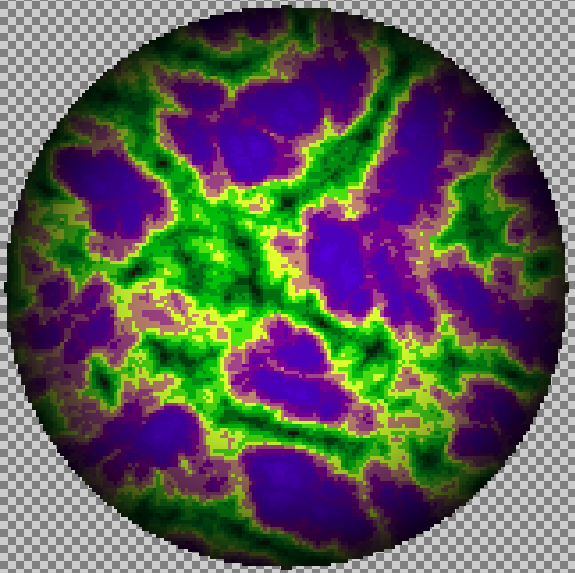
\includegraphics[scale=0.25]{blurInit.png}
        \caption{Avant floutage}
        \label{subfig:avantflou}
    \end{subfigure}
    \begin{subfigure}{0.46\linewidth}
    \centering
        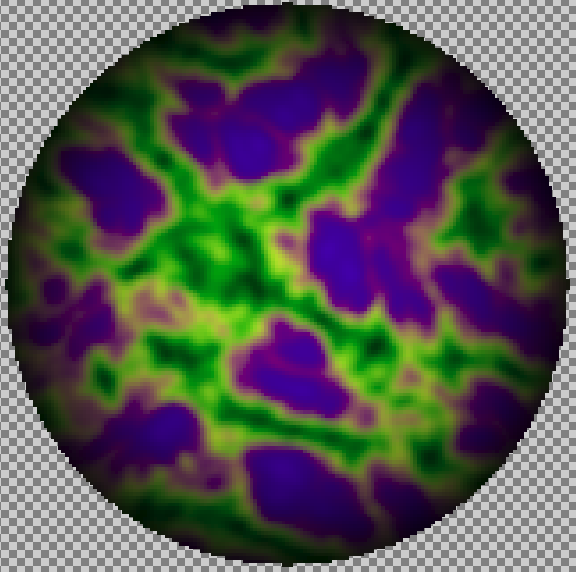
\includegraphics[scale=0.25]{blurFinal.png}
        \caption{Après floutage}
        \label{subfig:aprèsflou}
    \end{subfigure}
    \caption{Application du filtre Flou Gaussien}
    \label{fig:gaussian_blur}
\end{figure}

Pour conclure sur le filtre de flou Gaussien, nous pouvons dire qu'il est fonctionnel, cependant il n'est pas fonctionnel pure car il a nécessité la création d'un noyau dans une variable. Et donc il entraîne l'apparition d'effets de bords. Cependant, ces effets sont contrôlés car le noyau est manipulé une seule et unique fois.

\subsubsection{Filtre de symétrie}

Le filtre \texttt{mirror} est un filtre de symétrie qui permet der réaliser un effet de miroir et donc de retourner horizontalement ou verticalement une image. Ainsi, il nécessite plusieurs paramètres :
\begin{itemize}
    \item \texttt{src} La fonction de génération initiale
    \item \texttt{axe} Les axes de symétrie : $x$, $y$, ou $x$ et $y$
    \item \texttt{width, height} les dimensions de l'image en entrée afin d'en réaliser son retournement.
\end{itemize}

Ce filtre, à partir d'une fonction de génération d'un pixel aux coordonnées $(x,y)$, ne fait que retourner la fonction de génération d'un autre pixel, de façon symétrique par rapport aux axes de symétrie choisis. \\
Ainsi, ce filtre est purement fonctionnel, il n'entraîne aucun effet de bords.

\subsubsection{Filtre Clear}

Le filtre \texttt{clear} est un filtre qui n'affiche que certaines parties d'une image, laissant les autres transparentes. Ainsi le filtre est appelé sur des coordonnées $(x,y)$, et une fonction \texttt{toClear} qui à partir des coordonnées, décide si le pixel doit être affiché sur l'image ou non. \\

Par exemple, ce filtre appelé sur un pixel $(x,y)$ avec la fonction \texttt{toClear : (x,y) => \{true ? x \% 2 === 0; false\}} retourne la fonction de génération du pixel $(x,y)$ que lorsque ce dernier a une coordonnée $x$ paire. Sinon, le filtre retourne la fonction de génération du pixel transparent. \\

Ainsi ce filtre est implémenté en programmation fonctionnelle pure, car il ne créé aucune variable et donc aucun effet de bords.

\subsubsection{Filtre de renflement (Bulge)}

Le renflement d'une image consiste en sa modification de façon bombée ou au contraire contractée. Le filtre \texttt{bulge} est ainsi le filtre qui bombe ou contracte une image. Il prend en paramètre un coefficient de renflement. Si ce coefficient est négatif, alors l'image sera contractée et donc l'image retournée sera une implosion de l'image initiale. S'il est positif, alors l'image générée sera bombée et correspondra à une explosion de l'image initiale. Plus la valeur absolue du coefficient est important, et plus le renflement sera important (implosion ou explosion). \\

Le filtre prend donc plusieurs paramètres :
\begin{itemize}
    \item \texttt{src} La fonction génératrice de l'image en fonction des coordonnées
    \item \texttt{size} Un dictionnaire des dimensions de l'image initiale
    \item \texttt{bulge} Un dictionnaire des coordonnées centraux du renflement
    \item \texttt{coef} Le coefficient de renflement
\end{itemize}

Ainsi, il est possible de faire varier l'intensité du renflement mais également la position du renflement qui n'est pas obligatoirement au centre de l'image. \\

Nous avons choisi de ne pas implémenter ce filtre de façon fonctionnelle pure. En effet, cela aurait été possible, cependant la complexité de la fonction aurait grandement augmentée du fait du calcul multiple des mêmes valeurs.

\begin{figure}[H]
    \centering
    \begin{subfigure}{0.46\textwidth}
    \centering
        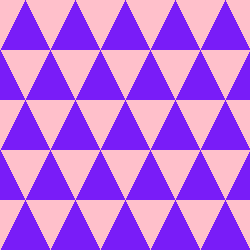
\includegraphics[scale=0.45]{bulgeInit.png}
        \caption{Avant explosion}
        \label{subfig:avantbulge}
    \end{subfigure}
    \begin{subfigure}{0.46\textwidth}
    \centering
        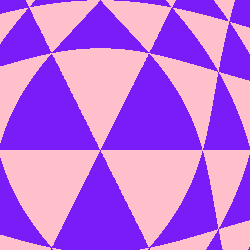
\includegraphics[scale=0.45]{bulgeFinal.png}
        \caption{Après explosion}
        \label{subfig:aprèsbulge}
    \end{subfigure}
    \caption{Application du filtre de renflement appelé sur une explosion}
    \label{fig:bulge}
\end{figure}

\subsubsection{Filtre de transformation, limitation et répétition}

Dans l'imagerie, les modifications principales appliquées sur les images sont les redimensionnements, les translations, et les rotations.
Nous avons donc implémenté un filtre qui gère ces trois transformations possible sur une image. \\

Le filtre \texttt{transform} utilise donc différents paramètres qui gèrent le redimensionnement, la translation et la rotation susceptibles d'être appliqués sur l'image :
\begin{itemize}
    \item \texttt{offset} Un dictionnaire comprenant les translations selon x et y
    \item \texttt{scale} L'échelle de redimensionnement de l'image en fonction des axes x et y par rapport à l'image de base
    \item \texttt{angle} L'angle de rotation de l'image \\
\end{itemize}

Ainsi le filtre prend en paramètre une fonction de génération d'une image en fonction de coordonnées, et renvoie celle de la même image mais à des coordonnées différentes en fonction des transformations appliquées. Par exemple, voici une image initiale et celle renvoyée après une rotation de 42°, une translation des $x$ de 50 pixels, de $y$ de 10 pixels et un redimensionnement de 0.5 selon les deux axes (l'image finale mesure donc 0.5 fois la taille de l'image initiale). \\

\begin{figure}[H]
    \centering
    \begin{subfigure}{0.46\textwidth}
    \centering
        
\includegraphics[scale=0.15]{transformInit.png}
        \caption{Avant transformation}
        \label{subfig:avanttrasnform}
    \end{subfigure}
    \begin{subfigure}{0.46\textwidth}
    \centering
        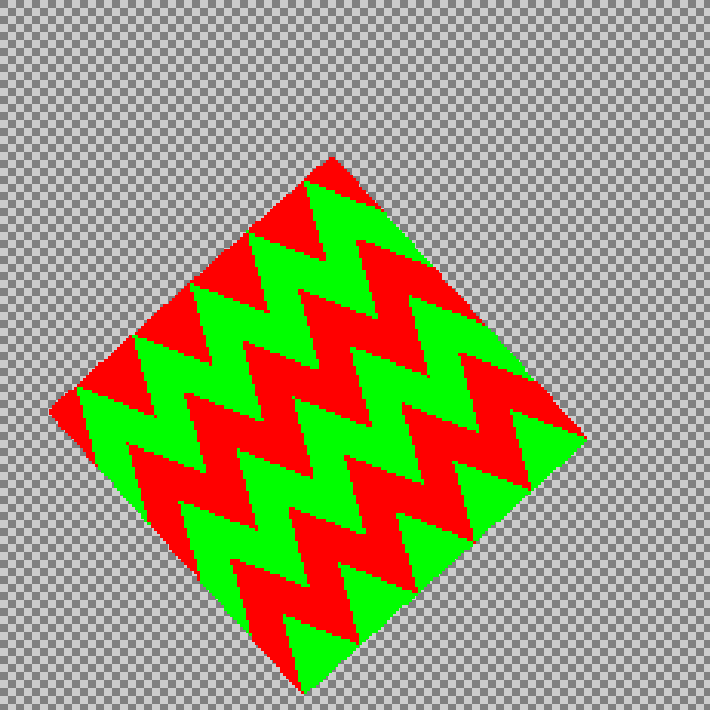
\includegraphics[scale=0.16]{transformFinal.png}
        \caption{Après transformation}
        \label{subfig:aprèstransform}
    \end{subfigure}
    \caption{Application du filtre de transformation}
    \label{fig:transform}
\end{figure}

Pour ce filtre également, par soucis de complexité, nous avons fait le choix de ne pas l'implémenter de façon fonctionnelle pure. Cependant, Chaque variable initialisée sont des constantes, elles ne sont pas manipulées par la fonction et ne servent qu'à éviter de recalculer plusieurs fois les mêmes valeurs et donc augmenter la complexité. Ainsi l'implémentation du filtre reste fonctionnelle. \\

D'une manière fonctionnelle pure, nous avons implémenté un second filtre, appelé filtre de limitation. Comme son nom l'indique, ce filtre limite la taille d'une image. Ainsi, il ne renvoie la fonction génératrice du pixel donnée en paramètre que si les coordonnées du pixel appartiennent à un certain intervalle $[x_{min}, x_{max}] * [y_{min}, y_{max}]$ lui aussi passé en paramètre. \\

Un troisième filtre similaire est le filtre de répétition. Ce filtre prend en paramètre les dimensions initiales de l'image, ainsi que des dimensions plus petites. Puis il réduit l'image initiale, et la répète jusqu'à ce que l'image obtenue soit de même dimensions que l'image initiale.

\subsubsection{Filtre de pixellisation}

Le filtre \texttt{pixelate} est un filtre de pixellisation d'une image. Ainsi, à partir d'une image de départ, il retourne une fonction de génération d'une image qui correspond à une version pixellisée de l'image initiale. \\
L'utilisation d'un unique paramètre \texttt{size} permet de redimensionner la taille d'un pixel sur l'image de façon à la pixelliser. Ainsi les pixels de l'image de sortie sont plus gros que ceux de l'image en entrée. \\
 
Ce filtre est purement fonctionnel. En effet, comme de nombreux autres effets, il ne fait que retourner la valeur d'un pixel déjà existant de l'image en fonction des coordonnées $(x,y)$ données en paramètre. \\
 
Par exemple, si la taille donnée en paramètre est $\{x:10, y:7\}$, alors les pixels seront regroupés par groupes rectangles de 10x7, ayant tous la même couleur, pour ne former qu'un unique gros pixel.
 
Voici un exemple de pixellisation d'une image :
 
\begin{figure}[H]
    \centering
    \begin{subfigure}{0.46\textwidth}
    \centering
        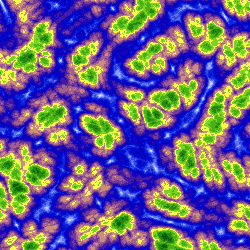
\includegraphics[scale=0.45]{pixelateInit.png}
        \caption{Avant pixellisation}
        \label{subfig:avantpixelate}
    \end{subfigure}
    \begin{subfigure}{0.46\textwidth}
    \centering
        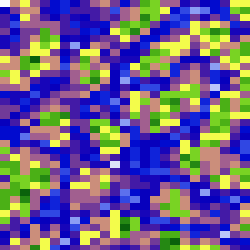
\includegraphics[scale=0.45]{pixelateFinal.png}
        \caption{Après pixellisation}
        \label{subfig:aprèspixelate}
    \end{subfigure}
    \caption{Application du filtre de pixellisation}
    \label{fig:pixelate}
\end{figure}
 
\subsubsection{Filtre de colorimétrie}
 
La colorimétrie est très importante en imagerie. Nous avons donc décidé d'implémenter différents filtres liés à cette notion. Le plus connu est le filtre noir et blanc. Mais nous avons également implémenté le filtre de négation, c'est-à-dire celui qui inverse la colorimétrie d'une image (les blancs deviennent des noirs et inversement, ...). De plus, un simple filtre \texttt{changeRGBAColor} a été implémenté afin de modifier les rouges, les verts, ou bien les bleus d'une image. \\
 
 Pour chacun de ces filtres, nous avons choisi de ne pas augmenter inutilement la complexité et donc avons utilisé une déclaration de constante pour ne pas avoir à recalculer la fonction à chaque fois. Ainsi, ils ne sont pas purement fonctionnels. Cependant, ils restent fonctionnels pour autant, car ils ne manipulent aucun effets de bords.

\subsubsection{Filtre 3D anaglyphe}

Un anaglyphe est une image prévue pour être vue en relief, à l’aide de deux filtres de couleurs différentes disposés devant chacun des yeux de l’observateur. Les anaglyphes se basent sur le décalage entre les deux yeux pour que le cerveau perçoivent le relief. Ainsi, le filtre \texttt{anaglyphe} est un filtre qui créé un décalage entre les rouges et les cyans d'une image de façon à créer un effet 3D perceptible à l'oeil nu et interprétable avec des lunettes 3D (rouge et bleu). \\

Ainsi, suivant les paramètres donnés, les rouges sont décalés d'une translation \texttt{dx} vers les $x$ positifs et \texttt{dy} dans le sens des $y$ positifs. Les cyan (vert et bleu) subissent la translation inverse. \\

\subsection{Filtres composés}

Les filtres composés sont des filtres qui à partir de deux fonctions génératrices de pixel, retourne une unique fonction, résultante de la composition des deux autres. Cette sous-section a pour but de détailler les différentes compositions possibles.

\subsubsection{Filtre d'opération}

Un premier filtre de composition est le filtre d'opération. C'est un filtre qui à partir de deux fonctions génératrices de pixel, retourne une unique fonction de génération d'un pixel. Ce pixel résulte alors de l'opération donnée en paramètre. \\

\noindent Par exemple, si on appelle le filtre sur une image \texttt{src} et sur une image \texttt{dst} avec l'opération \texttt{(a,b) => a*b + b}, alors pour chaque composante du pixel R, G, B et A, le filtre va effectuer l'opération et va retourner une fonction génératrice avec la nouvelle couleur.
Ainsi sur l'exemple, la fonction retournée sera la fonction génératrice de la couleur :
$$\big( R_a*R_b+R_b,~ G_a*G_b+G_b,~ B_a*B_b+B_b,~ A_a*A_b+A_b \big)$$

Il est possible d'appeler ce filtre avec de nombreuses opérations. Ainsi nous avons créer 5 nouveaux filtres de composition qui reposent sur ce filtre d'opération.

\subsubsection{Filtre add, minus, multiply, divide, screen}

Ces filtres reposent tous sur le filtre \texttt{operation}. En effet, ces cinq filtres prennent en paramètre deux fonctions de générations de pixel, et appellent le filtre d'opération pour retourner une unique fonction. Ainsi, ils sont purement fonctionnels car ils ne font que retourner un autre filtre, lui-même fonctionnel. \\

Le filtre \texttt{add} appelle le filtre opération sur une addition de la première fonction et la deuxième. \\

Le filtre \texttt{minus} l'appelle sur une soustraction de la première par la deuxième. L'ordre des fonctions données en paramètre est donc important ici. Cependant, si la deuxième composante est supérieure à la première, alors la valeur renvoyée est 0. En effet les composantes des pixels sont comprises entre 0 et 255. \\

Le filtre \texttt{multiply} renvoie par le même procédé la multiplication des composantes des pixels. Pour réaliser cette mutliplication, le filtre multiplie les composantes entre elles, puis divise le résultat par 255 pour se ramener à la couleur d'un pixel comprise entre 0 et 255. \\

\begin{figure}[H]
    \centering
    \begin{subfigure}{0.3\textwidth}
    \centering
            
\includegraphics[width=4cm]{multiplyInit1.png}
        \caption{\'Echiquier}
        \label{fig:chessboard}
    \end{subfigure}
    \begin{subfigure}{0.3\textwidth}
    \centering
        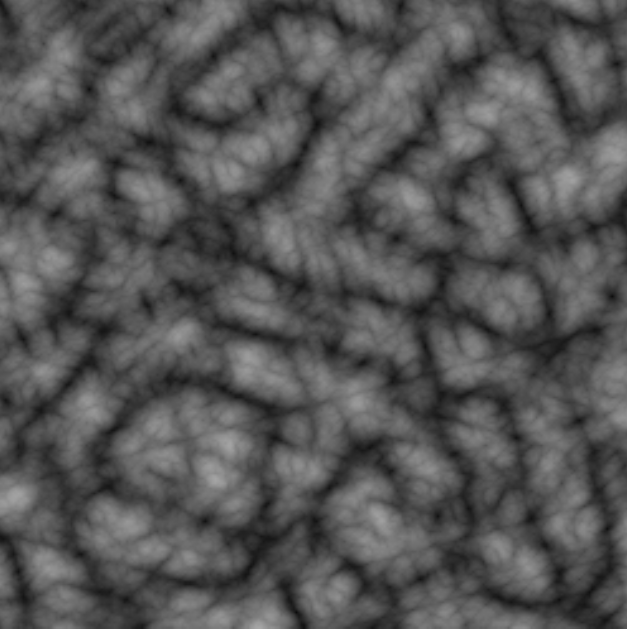
\includegraphics[width=4cm]{multiplyInit2.png}
        \caption{Bruit de Perlin}
        \label{fig:perlinnoise}
    \end{subfigure}
    \begin{subfigure}{0.3\textwidth}
    \centering
        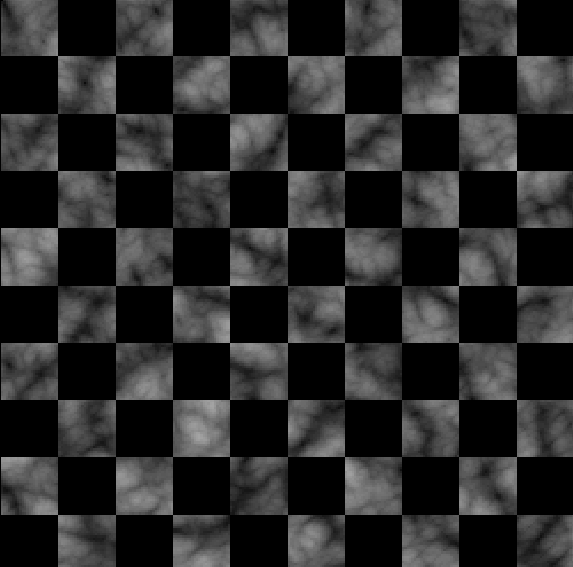
\includegraphics[width=4cm]{multiplyFinal.png}
        \caption{Composition de type multiply}
        \label{fig:chessboard_x_perlin_noise}
    \end{subfigure}
    \caption{Exemple de composition de type \textit{multiply} entre un échiquier et un bruit de Perlin avec turbulences}
    \label{fig:multiply}
\end{figure}

Le filtre \texttt{screen} est une variante du filtre de multiplication. En effet, il réalise le produit entre deux images. Cependant, il passe les images en négatifs avant de les multiplier, puis il repasse le résultat en négatif pour retomber sur les couleurs initiales. \\

Le filtre \texttt{divide} renvoie de la même manière la division des composantes renvoyées par la deuxième fonction donnée en paramètre par celle renvoyées par la première fonction. Pour réaliser cette division, le filtre effectue l'opération $\big((b+1)/(a+1)\big)*255$. En effet, les pixels sont compris entre 0 et 255, il est donc nécessaire d'ajouter 1 pour éviter les divisions par 0. Puis il faut multiplier par 255 pour se ramener à la plage de données d'un pixel. \\

\begin{figure}[H]
    \centering
    \begin{subfigure}{0.3\textwidth}
    \centering
            \includegraphics[width=4cm]{fractal-Worley.png}
        \caption{Bruit fractal de worley}
        \label{fig:fractal-Worley}
    \end{subfigure}
    \begin{subfigure}{0.3\textwidth}
    \centering
        \includegraphics[width=4cm]{voronoi-random.png}
        \caption{Pavage voronoi aléatoire}
        \label{fig:voronoi-rng}
    \end{subfigure}
    \begin{subfigure}{0.3\textwidth}
    \centering
        \includegraphics[width=4cm]{fractal-Worley-divide-voronoi.png}
        \caption{Composition de type divide}
        \label{fig:voronoi-fractal-Worley}
    \end{subfigure}
    \caption{Exemple de composition de type \textit{divide} entre un générateur voronoi aléatoire et un bruit fractal de worley}
    \label{fig:divide}
\end{figure}

\subsubsection{Autre compositions}

En plus des opérations, il existe des compositions connues sur les images. Par exemple, nous avons implémenté les compositions qui retournent la fonction de génération de la première image donnée en paramètre mais avec l'opacité de la deuxième. Ou encore, le filtre qui retourne la première image en paramètre mais avec une opacité de sortie qui vaut $255 - opacite$ avec $opacite$ l'opacité de la deuxième image. \\

Le filtre \texttt{atop} est similaire. C'est à dire qu'il retourne un pixel composé de la composition src de la deuxième image par la première données en paramètres à condition que les deux opacités soient positives. Si celle de la première image donnée en paramètre, alors le filtre retourne un pixel transparent. Si c'est la deuxième image qui possède une opacité nulle, alors le filtre retourne le pixel généré par la première image. \\

Le filtre \texttt{xor} est également un filtre de composition. Il prend chaque composante de chaque pixel de chaque image, et il renvoie la composante égale au \textit{ou exclusif} des deux composantes initiales. Ainsi, l'image formée en retour de cette fonction est un "ou exclusif" des deux images données en paramètres.

Enfin, le filtre \texttt{over} est également un filtre de composition que nous avons implémenté. Ce filtre réalise la superposition de deux images. C'est-à-dire qu'il prend la première et il la positionne par dessus la deuxième. Cependant, les opacités multipliées par des coefficients qui dépendent des opacités initiales, permettent de ne pas avoir une unique superposition mais bien un mélange des deux images. Ainsi, ce filtre ressemble au filtre d'addition cependant, il prend en compte les opacités pour que la première image domine légèrement sur la deuxième. \\

En dehors de la déclaration de constantes pour éviter une complexité trop importante, ces filtres sont fonctionnels car ils ne manipulent aucun effets de bords et ils ne font que retourner une fonction de génération d'un pixel en fonction des deux fonctions données en paramètres.
De plus, ils sont purs. Ils ne modifient pas le ou les images données en entrées. Qui plus est, ils retournent une nouvelle image.  

\newpage
\section{Tests}
Afin de vérifier la cohérence de nos implémentations de générateurs et de filtres, il est nécessaire de les tester. Ainsi, on s'assure de leur bon fonctionnement sur nos images. Pour cela, nous avons utilisé l'outil \texttt{jest} qui réalise des tests à l'aide d'assertions. De plus cet outil calcul le taux de couvertures de nos fonctions par nos tests. Il est donc un bon facteur pour vérifier que l'entièreté de notre implémentation a été testée. Cette section a pour but d'illustrer la façon dont nous avons implémenté nos tests.

\subsection{Tests des générateurs}

\subsubsection{Tests des générateurs de bruit spatial}

Comme nous avons pu le spécifier précédemment dans la section \ref{section:noiseGenerationIntro}, les valeurs de la fonction retournée par le générateur de bruit \texttt{noiseGenerator} dépendent de l'ordre d'exécution de cette dernière. Cependant, toute suite identique d'exécution conduit à une suite de résultats strictement identiques. C'est ce principe qui a été utilisé afin de tester le bon fonctionnement des différents modules de génération de bruit spatial.

Ainsi, les tests ont consisté à faire des tests du type entrées/sorties. Ces derniers ont été réalisés à travers l'utilisation de seed, permettant ainsi une exécution équivalente des tests dans le temps, et permettre la non-régression des tests. Afin de vérifier la texture issu de la génération de ces bruits, une vérification à travers sept coordonnées éparpillées dans une grille de $250$x$250$ est effectuée par comparaison au résultat attendu (de valeur de bruit ou de couleur du pixel). Ainsi, bien que ne représentant pas la texture finale, cette suite d'exécution permet de tester le comportement général du bruit par l'intermédiaire de cas représentatifs de l'exécution finale.

Ainsi, une fois la réalisation d'un code initial ayant un fonctionnement tel qu'attendu, l'écriture de tests a été réalisée, permettant ainsi de comparer le comportement de toutes modifications avec celui d'un valide. Par ailleurs, ce type de test permet d'éviter une génération complète de la texture, et ainsi permet d'obtenir des tests rapides et efficaces lors du développement de nouvelles fonctionnalités ou modification du code initial.

Enfin, l'exécution de ces tests à travers \textit{generators.test.js} a permis de couvrir $100\%$ du code de \textit{noiseGenerators.js}, et ainsi de vérifier le fonctionnement de l'ensemble des générateurs de bruit spatial. Ces tests ont été particulièrement utiles lors du réusinage ("refactoring" en anglais) du code, afin de le rendre plus en symbiose avec les principes de la programmation fonctionnelle.

\subsubsection{Tests des générateurs de pavages et des générateurs de gradients}

L'implémentation des générateurs de pavages et de gradients ne dépend que de règles mathématiques et géométriques. De plus, l'ordre d'exécution sur les différents pixels n'influence pas sur l'évaluation de nos générateurs grâce à leur pureté. Afin de tester ces générateurs, nous avons pris un échantillon de pixels et vérifié si la couleur renvoyée par le générateur pour chacun des pixels de l'échantillon correspondait à la couleur théorique.

\subsection{Tests des filtres}

Les tests des filtres sont nécessaires pour s'assurer de leur bonne implémentation et également qu'ils réalisent bien les modifications attendues sur les images. Nous obtenons une couverture de 97.34\% lors de l'exécution des tests sur les filtres ce qui est satisfaisant pour assurer leur bonne implémentation. Cette partie illustre la manière dont nous avons choisi d'implémenter nos tests sur les filtres.

\subsubsection{Tests des filtres non-composés}

Les filtres non-composés étant des fonctions prenant en paramètre une fonction de génération et renvoyant une fonction de génération modifiée, nous avons implémenté les tests de la façon suivante. Nous appelons un générateur d'image parmi nos générateurs, puis nous le filtrons avec l'un des filtres implémentés. Ensuite, il suffit de vérifier la version filtrée en regardant si elle correspond bien à la bonne version modifiée de la version non-filtrée. \\

Pour cela, nous testons un échantillon de pixels filtrés et on les compare au pixel non-filtrés sur lesquels nous appliquons nous même la transformation souhaitée.

\subsubsection{Tests des filtres composés}

La façon de tester les filtres composés est la même que pour les filtres non-composés. Cependant, il est nécessaire d'appeler deux générateurs en entrée, et de comparer le pixel en sortie avec le résultat attendu en fonction des deux pixels en entrée.

\newpage
\section{Gestion de projet}
\label{section:project-management}

Dans cette section, nous présentons la manière dont nous avons managé le projet en terme de répartition des tâches ainsi que les améliorations possibles. \\

Notre première approche a consisté à ce que chacun écrive ses propres filtres et générateurs en ayant comme seule contrainte le respect de la représentation d'une image, d'un générateur et d'un filtre tel que nous l'avions décidé. \\

Nous avons rapidement changé d'organisation afin d'éviter les dérives de projets et la duplication de tâches. Nous nous sommes ainsi répartis les différents générateurs et filtres à créer ainsi que par conséquence les responsabilités. La répartition finale des tâches est la suivante : 
\begin{itemize}
\item CHOURA Alexandre : programmeur des générateurs de bruits spatiaux;
\item GUÉRIN Léo : programmeur des générateurs de pavages et des gradients de couleurs;
\item MARAIS Lucas : programmeur attitré aux filtres;
\item SORNAY Jean-François : coordinateur du projet, programmeur de filtres et réusineur du code. \\
\end{itemize}

Cette répartition fut nécessaire afin d'éviter des problèmes de duplication de code et de communication. Cela nous a permis d'avancer avec une meilleure dynamique avec moins de conflits d'implémentation et de faire du \textit{refactoring} plus rapidement quand c'était nécessaire. \\

Cependant, ce changement est arrivé un peu tard car nous n'avons pas pris le temps d'analyser correctement les tenants et les aboutissants du projet. Cela nous a fait défaut lors de la mise en commun.

\newpage
\section{Conclusion}

La réalisation du projet de génération procédurale nous a permis de travailler en équipe, contrairement au projet du semestre 5, nous étions 4. La coordination était donc beaucoup plus importante, et nous l'avons rapidement mise en place. L'objectif du projet qui était la génération d'image de façon fonctionnelle était mené à bien avec l'implémentation de générateurs et filtres, ainsi que la génération d'un fichier \texttt{html} et \texttt{png}. \\

\'Egalement, la mise en place de générateurs et filtres complexes a pris une place importante dans ce projet. Cela nous a permi d'améliorer nos compétences en programmation fonctionnelle. En effet, la complexité du projet résidait dans le caractère fonctionnel des générateurs et filtres mis en place. Nous avons, autant que possible établit des fonctions fonctionnelles pures. Cependant, nous avons fait certains choix pour améliorer la complexité de certaines fonctions, en diminuant la pureté de certains filtres ou générateurs par exemple. \\

La continuité du projet aurait été dans l'élaboration d'une interface graphique fonctionnelle en html. Ainsi, la manipulation d'images aurait été simplifiée par le choix d'un générateur, puis l'application de filtres directement sur la page html. C'est sur ce point que nous aurions essayé d'améliorer notre projet. De plus, nous avions pensé, lors de l'élaboration de nos différents générateurs et filtres dans le fichier \texttt{image.js}, à la possibilité de lire un fichier au format \texttt{JSON} permettant la génération d'une image particulière. Cependant, nous n'avons pas eu le temps d'exploiter pleinement cette possibilité. Cela pourrait être un axe d'amélioration. \'Egalement, l'implémentation de nouveaux générateus et nouveaux filtres reste une piste d'amélioration du projet. \\

Ce projet a donc été un excellent moteur pour se familiariser avec la notion de pureté, et améliorer nos connaissance en programmation fonctionnelle. De plus, la manipulation de Javascript, avec le linkage de plusieurs fichiers entre-eux notamment, nous a permit d'accroître nos connaissances. \\

\newpage
\nocite{*}
\bibliography{main} 
\bibliographystyle{ieeetr}

\end{document}
